\documentclass[12pt]{journal}
\usepackage[a4paper, total={6in, 8in}]{geometry}
\usepackage[utf8]{inputenc}
\usepackage{float}
\usepackage{graphicx}
\usepackage{amsmath}

\title{UNIT 3 : PEMODELAN SISTEM}
\author{ALIM SATRIA FI'I WIJAYA KUSUMA (21/483503/SV/20304)}
\date{March 2022}

\begin{document}

\maketitle

\section{Rangkuman singkat materi}

Dalam identifikasi sistem, sangat penting untuk bisa mengetahui dan mempelajari sifat dari sebuah sistem. Hal yang dapat dilakukan untuk mengetahui dan mempelajari sifat sebuah sistem dapat dilakukan dengan memodelkan sistem tersebut secara matematis berdasarkan sifat komponen penyusun sistem tersebut. Hasil dari pemodelan tersebut disebut sebagai transfer function. Dengan transfer function, dapat diketahui sifat respon sistem terharap masukan yang diberikan melalui keluaran sistem. Melalui analisis dari sistem tersebut dapat dilakukan penalaan terhadap sistem agar perilaku sistem sesuai dengan yang diharapkan.

\section{Latihan}

\subsection{Pemodelan motor listrik}

Percobaan pertama merupakan pemodelan motor DC dengan simulink seperti yang ditunjukkan pada gambar satu, respon sistem dari motor DC dapat dilihat pada gambar dua.

\begin{figure}[H]
    \centering
    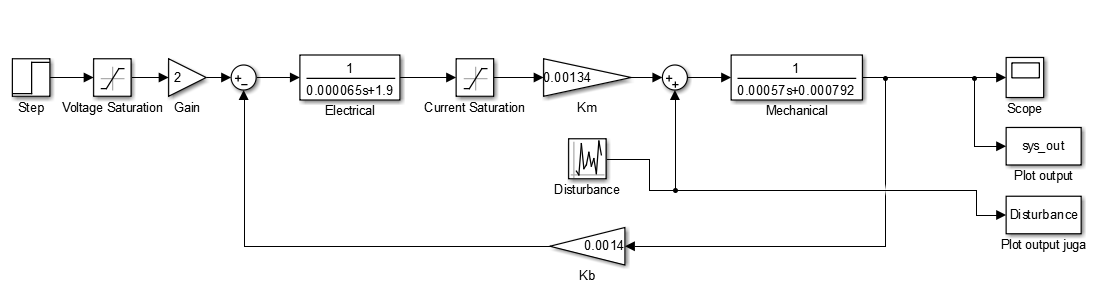
\includegraphics[width=\textwidth]{soal_nomor_1.png}
    \caption{Model simulink motor DC}
    \label{simulink_motor_DC}
\end{figure}

Berdasarkan respon sistem yang ada pada gambar dua dapat terlihat bahwa gangguan (\textit{disturbance}) memiliki pengaaruh yang besar dalam keluaran dari sebuah sistem. Karena adanya disturbance menyebabkan sistem tidak mampu mencapai \textit{steady state}. Disturbance juga membuat sistem tidak mampu mencapai setpoint karena sistem tidak stabil.

\begin{figure}[H]
    \centering
    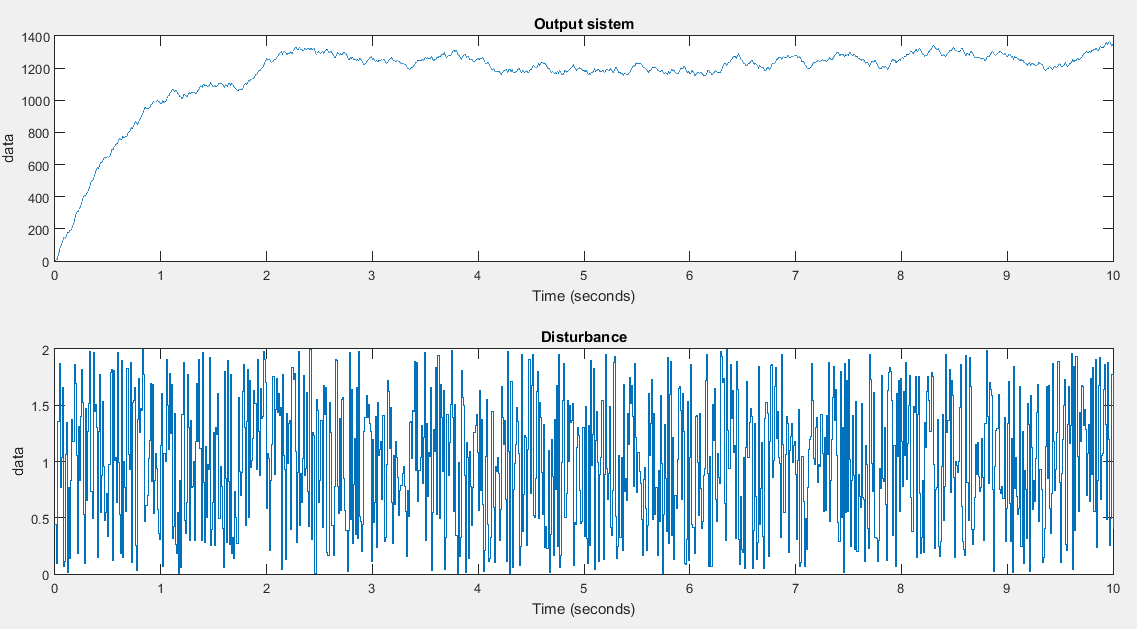
\includegraphics[width=\textwidth]{hasil_nomor_1.png}
    \caption{Hasil simulasi simulink}
    \label{soal_nomor_satul}
\end{figure}

\pagebreak

\subsection{Permodelan orde satu dan orde dua}

Pada gambar tiga, terlihat perbandingan antara respon sistem dengan orde satu dan respon sistem dengan orde dua. Dari respon tersebut dapat dilihat bahwa sistem dengan orde dua memiliki \textit{rise time} yang sedikit lebih cepat daripada sistem orde satu dengan kesetabilan sistem yang sama.

\begin{figure}[H]
    \centering
    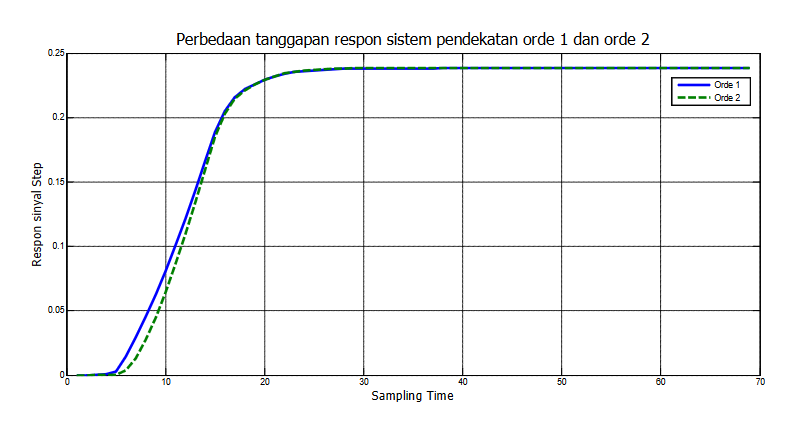
\includegraphics[width = \textwidth]{soal_nomor_2.png}
    \caption{Perbandingan respon sistem orde satu dan orde dua}
    \label{hasil_nomor_satu}
\end{figure}

\subsection{Latihan model 3}

\begin{figure}[H]
    \centering
    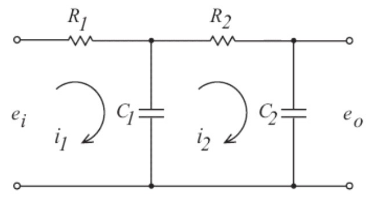
\includegraphics{model_nomor_3.png}
    \caption{Rangkaian RC dua loop}
    \label{soal_nomor_3}
\end{figure}

Pemodelan ini dapat diselesaikan dengan memodelkan rangkaian listrik masing-masing loop pada sistem, model pada loop urut dari sebelah kiri ($e_i$) dinyatakan sebagai berikut,

\begin{equation*}
    \begin{split}
        e_{i} &= V_{R1} + V_{C1} \\[5pt]
        E_{i} &= I_{1}R_{1} + \frac{1}{C_{1}s}[I_{1}-I_{2}]
    \end{split}
\end{equation*}

persamaan diatas dapat disusun ulang untuk untuk mendefinisikan nilai $ I_{1} $  sebagai berikut,

\begin{equation}
    I_1 = \frac{E_iC_1s+I_2}{R_1C_1s+1}
\end{equation}

Selanjutnya, dapat dilakukan perhitungan untuk mengetahui persamaan pada bagian loop tengah rangkaian sebagai berikut,

\begin{equation*}
    \begin{split}
        0 & = V_{R2} + V_{C2} + V_{C1} \\[5pt]
        0 & = I_2R_2 + \frac{1}{C_2s}I_2 + \frac{1}{C_1s}[I_2-I_1]
    \end{split}
\end{equation*}

Persamaan diatas dapat disederhanakan kembali sebagai berikut,

\begin{equation}
    \begin{split}
        0 &= I_2\underbrace{[R_2+\frac{1}{C_1s}+\frac{1}{C_2s}]}_{\text{X}}-I_1\underbrace{[\frac{1}{C_1s}]}_{\text{Y}}\\[5pt]
        0 &= I_2[X]-I_1[Y]
    \end{split}
\end{equation}

Persamaan ketiga merupakan persamaan rangkaian pada bagian $e_o$, persamaan tersebut dapat ditulis sebagai berikut,

\begin{equation*}
    \begin{split}
        e_o &= V_{C2} \\[5pt]
        E_o &= \frac{1}{C_2s}I_2
    \end{split}
\end{equation*}

persamaan diatas dapat disusun ulang untuk mendapatkan nilai $I_2$ menjadi persamaan berikut,

\begin{equation}
    I_2 = C_2sE_o
\end{equation}

untuk mendapatkan transfer function dari model, maka persamaan satu dan persamaan tiga dapat dimasukkan pada persamaan dua sebagai berikut,

\begin{equation*}
    \begin{split}
        0 &= I_2[X]-I_1[Y] \\[5pt]
        0 &= C_2sE_o[X]-\frac{E_iC_1s+C_2sE_o}{R_1C_1s+1}[Y] \\[5pt]
        0 &= C_2sE_o[X]-\frac{E_iC_1s}{R_1C_1s+1}[Y]-\frac{C_2sEo}{R_1C_1s+1}[Y] \\[5pt]
        \frac{E_iC_1s}{R_1C_1s+1}[Y] &= \frac{[C_2sE_o]R_1C_1s+1}{R_1C_1s+1}[X]-\frac{[C_2sE_o]}{R_1C_1s+1}[Y] \\[5pt]
        E_iC_1s[Y] &= C_2sE_o[[R_1C_1s+1][X]-[Y]]
    \end{split}
\end{equation*}

Persamaan diatas dapat disederhanakan kedalam bentuk berikut,

\begin{equation}
    \frac{E_iC_1s[Y]}{C_2sE_o} = [R_1C_1s+1][X]-[Y]
\end{equation}

Setelah diperoleh persamaan empat, langkah berikutnya adalah memasukkan nilai $X$ dan nilai $Y$ ke persamaan tersebut,

\begin{equation*}
    \begin{split}
        \frac{E_iC_1s[\frac{1}{C_1s}]}{E_oC_2s} &= [R_1C_1s+1][R_2+\frac{1}{C_1s}+\frac{1}{C_2s}]-[\frac{1}{C_1s}] \\[5pt]
        \frac{E_i}{E_oC_2s} &= R_1R_2C_1s+R_1C_1\frac{1}{C_2s}+R_1+R_2+\frac{1}{C_2s} \\[5pt]
        \frac{E_i}{E_o} &= R_1R_2C_1sC_2s+R_1C_1s+R_1C_2s+R_2C_2s+1
    \end{split}
\end{equation*}

Dari persamaan diatas didapat transfer function dari model sebagai berikut,

\begin{equation}
    \frac{E_o}{E_i} = \frac{1}{R_1R_2C_1C_2s^2+[R_1C_1+R_1C_2+R_2C_2]s+1}
\end{equation}

\pagebreak

\subsection{Latihan Model 4}

\begin{figure}[H]
    \centering
    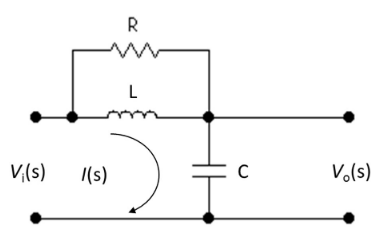
\includegraphics{model_nomor_4.png}
    \caption{Pemodelan rangkaian RLC}
    \label{soal_nomor_4}
\end{figure}
 
 Transfer function untuk model RLC diatas dapat diketahui dengan mencari persamaan pada $V_i$ dan $V_o$. Persamaan pada $V_i$ dituliskan sebagai berikut,
 
 \begin{equation}
     \begin{split}
         V_i &= V_{RL}+V_C \\[5pt]
         V_i &= [\frac{1}{R}+\frac{1}{Ls}]I+[\frac{1}{Cs}]I
     \end{split}
 \end{equation}
 
 Persaaman enam dapat disederhanakan kembali sebagai berikut,
 
 \begin{equation*}
     \begin{split}
         V_i &= [\frac{1}{R}+\frac{1}{Ls}]I+[\frac{1}{Cs}]I \\[5pt]
         V_i &= [\frac{RLs}{R+Ls}]I+[\frac{1}{Cs}]I
     \end{split}
 \end{equation*}
 \begin{equation}
     V_i = [\frac{RLs}{R+Ls}+\frac{1}{Cs}]I
 \end{equation}
 
 Setelah mencari persamaan pada bagian $V_i$, langkah  berikutnya adalah mencari persamaan pada bagian $V_o$ sebagai berikut,
 
 \begin{equation}
     \begin{split}
         V_o &= V_C \\[5pt]
         V_o &= \frac{1}{Cs}I
     \end{split}
 \end{equation}
 
 Dari hasil persamaan delapan dapat persamaan dapat disusun ulang untuk mendefinisikan $I$ sebagai berikut,
 
 \begin{equation}
     I = CsV_o
 \end{equation}
 
 Untuk memperoleh transfer function, persamaan sembilan disubtitusikan ke persamaan 
 tujuh sebagai berikut,
 
 \begin{equation*}
     \begin{split}
         V_i &= [\frac{RLs}{R+Ls}+\frac{1}{Cs}]I \\[5pt]
         V_i &= [\frac{RLs}{R+Ls}+\frac{1}{Cs}]CsV_o \\[5pt]
         V_i &= [\frac{RLsCs+[R+Ls]}{RCs+LsCs}]CsV_o \\[5pt]
         \frac{V_i}{V_o} &= [\frac{RLsCs+R+Ls}{[R+Ls]Cs}]Cs
     \end{split}
 \end{equation*}
 
 Dari persamaan diatas didapatkan transfer function sebagai berikut,
 
 \begin{equation}
     \frac{V_o}{V_i} = \frac{R+Ls}{RLCs^2+Ls+R}
 \end{equation}
 
\subsection{Latihan Model 5}
 
 \begin{figure}[H]
     \centering
     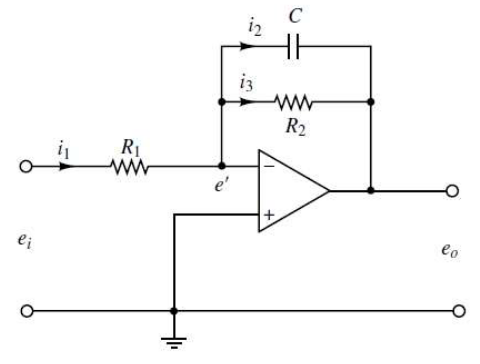
\includegraphics{model_nomor_5.png}
     \caption{Pemodelan Inverting OP-Amp}
     \label{soal_nomor_5}
 \end{figure}
 
 Transfer function untuk model diatas dapat dicari dengan memodelkan rangkaian pada arus yang masuk dan keluar dari OP-Amp, yaitu arus $i_1,i_2,$ dan $i_3$ sebagai berikut,
 
 \begin{equation}
     \begin{split}
         i_1 &= \frac{e_i-e'}{R_1} \\[5pt]
         i_2 &= C[\frac{e'-e_o}{dt}] \\[5pt]
         i_3 &= \frac{e'-e_o}{R_2}
     \end{split}
 \end{equation}
 
 Setelah mengetahui persamaan arus yang mengalir pada masing-masing komponen, langkah selanjutnya adalah mencari transfer function sistem menggunakan hukum kirchoff yang menyatakan bahwa jumlah arus yang masuk sama dengan jumlah arus yang keluar. Sehingga dapat dirumuskan sebagai berikut,
 
 \begin{equation*}
     i_1 = i_2+i_3
 \end{equation*}
 Berdasarkan hukum kirchoff diatas maka persamaan sebelas dapat dimasukkan menjadi,

 \begin{equation*}
    \frac{e_i-e'}{R_1}=C[\frac{e'-e_o}{dt}]+\frac{e'-e_o}{R_2}
 \end{equation*}
 
 Dalam keadaan ideal $e'$ bernilai nol. Sehingga,
    
\begin{equation*}
    \begin{split}
        \frac{e_i-0}{R_1} &= C[\frac{0-e_o}{dt}]+\frac{0-e_o}{R_2} \\[5pt]
        \frac{e_i}{R_1} &= C[\frac{-e_o}{dt}]+\frac{1}{R_2}[-e_o] \\[5pt]
        \frac{E_i}{R_1} &= -CsE_o-\frac{1}{R_2}E_o \\[5pt]
        \frac{E_i}{R_1} &= -[Cs+\frac{1}{R_2}]E_o \\[5pt]
        \frac{E_i}{E_o} &= -[Cs+\frac{1}{R_2}]R_1 \\[5pt]
        \frac{E_i}{E_o} &= -[R_1Cs+\frac{R_1}{R_2}]
    \end{split}
\end{equation*}
    
Dari persamaan tersebut, dapat diubah dan disederhanakan sebagai berikut,

\begin{equation*}
    \begin{split}
        \frac{E_o}{E_i} &= -\frac{1}{R_1Cs+\frac{R_1}{R_2}} \\[5pt]
        \frac{E_o}{E_i} &= -\frac{1}{R_1Cs+\frac{R_1}{R_2}} \frac{\frac{R_2}{R_1}}{\frac{R_2}{R_1}} \\[5pt]
    \end{split}
\end{equation*}
\begin{equation}
    \frac{E_o}{E_i} = -\frac{R_2}{R_1} \frac{1}{R_2Cs+1}
\end{equation}

\pagebreak

\subsection{Latihan model 6}

\begin{figure}[H]
    \centering
    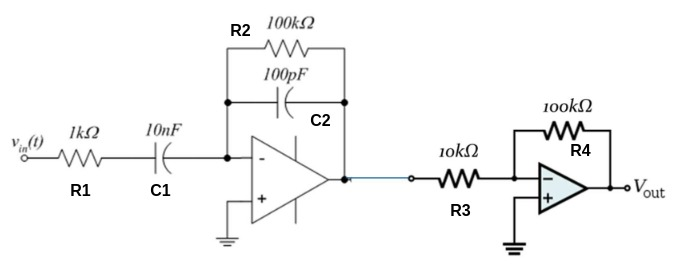
\includegraphics[width=\textwidth]{model_nomor_6.jpg}
    \caption{Rangkaian dua OP-Amp}
    \label{soal_nomor_6}
\end{figure}

untuk mendapatkan transfer function dari rangkaian diatas, harus dimodelkan terlebih dahulu persamaan impedansinya sebagai berikut,

\begin{equation}
    \begin{split}
        Z_1 &= \frac{R_1C_1s+1}{C_1s} \\[5pt]
        Z_2 &= \frac{R_2}{R_2C_1s+1} \\[5pt]
        Z_3 &= R_3 \\[5pt]
        Z_4 &= R_4
    \end{split}
\end{equation}

Setelah mendapatkan model impedansi, langkah selanjutnya adalah mencari transfer function pada OP-Amp pertama,

\begin{equation*}
    \begin{split}
        \frac{V'}{V_{in}} &= -\frac{Z_2}{Z_1} \\[5pt]
        \frac{V'}{V_{in}} &= -\frac{\frac{R_2}{R_2C_1s+1}}{\frac{R_1C_1s+1}{C_1s}} \\[5pt]
        \frac{V'}{V_{in}} &= -\frac{R_2C_1s}{R_1R_2C_1C_2s^2+[R_1C_1+R_2C_2]s+1}
    \end{split}
\end{equation*}
\begin{equation}
    V' = -\frac{R_2C_1s}{R_1R_2C_1C_2s^2+[R_1C_1+R_2C_2]s+1}V_{in}
\end{equation}

Persamaan empat belas dapat dimasukkan ke pemodelan OP-Amp kedua untuk memperoleh transfer function sistem,

\begin{equation*}
    \begin{split}
        \frac{V_{out}}{V'} &= -\frac{Z_2}{Z_1} \\[5pt]
        \frac{V_{out}}{V'} &= -\frac{R_4}{R_3} \\[5pt]
        V_{out} &= -\frac{R_4}{R_3}V' \\[5pt]
        V_{out} &= [-\frac{R_4}{R_3}][-\frac{R_2C_1s}{R_1R_2C_1C_2s^2+[R_1C_1+R_2C_2]s+1}V_{in}] \\[5pt]
        V_{out} &= \frac{R_4}{R_3}\frac{R_2C_1s}{R_1R_2C_1C_2s^2+[R_1C_1+R_2C_2]s+1}V_{in} \\[5pt]
    \end{split}
\end{equation*}

Persamaan diatas dapat disederhanakan menjadi transfer function sebagai berikut,

\begin{equation}
    \frac{V_{out}}{V_{in}}= \frac{R_4}{R_3}\frac{R_2C_1s}{R_1R_2C_1C_2s^2+[R_1C_1+R_2C_2]s+1} \\[5pt]
\end{equation}

Nilai dari masing-masing komponen kemudian disubtitusikan ke persamaan lima belas,

\begin{equation*}
    \begin{split}
        \frac{V_{out}}{V_{in}} &= \frac{[100k\Omega]}{[10k\Omega]}\frac{[100k\Omega][10nF]s}{[1k\Omega][100k\Omega][100pF]s^2+[[1k\Omega][10nF]+[100k\Omega][100pF]]s+1} \\[5pt]
        \frac{V_{out}}{V_{in}} &= \frac{10^{-3}}{10^{-2}s^2+[10^{-6}+10^{-5}]s+1}
    \end{split}
\end{equation*}

\pagebreak

\subsection{Step response sistem}

Pada percobaan terakhir, dilakukan simulasi pemberian step function pada pemodelan sistem dalam transformasi laplace, hasil pemodelan dapat dilihat sebagai berikut,

\subsubsection{fungsi satu}

\begin{figure}[H]
    \centering
    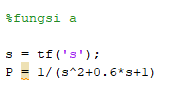
\includegraphics{7_a.png}
    \caption{Program M-file fungsi a}
    \label{soal_a}
\end{figure}
\begin{figure}[H]
    \centering
    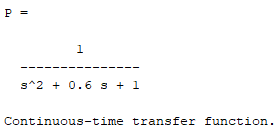
\includegraphics{hasil_7_a.png}
    \caption{Keluaran console MATLAB dari program fungsi a}
    \label{hasil_a}
\end{figure}

\subsubsection{fungsi dua}

\begin{figure}[H]
    \centering
    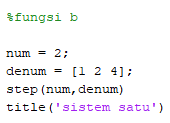
\includegraphics{7_b.png}
    \caption{Program M-file fungsi b}
    \label{soal_b}
\end{figure}
\begin{figure}[H]
    \centering
    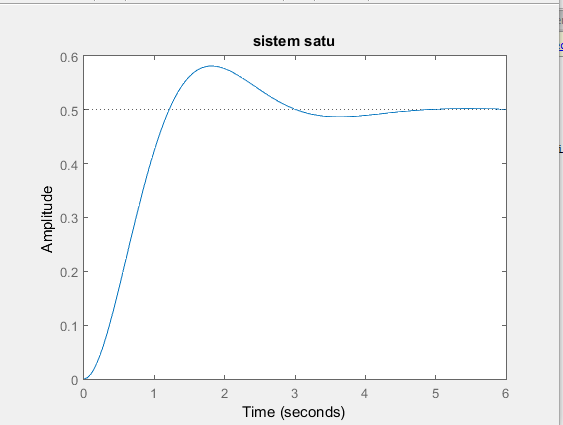
\includegraphics[width=\textwidth]{hasil_7_b.png}
    \caption{Keluaran plot MATLAB dari program fungsi b}
    \label{hasil_b}
\end{figure}

\subsubsection{fungsi tiga}

\begin{figure}[H]
    \centering
    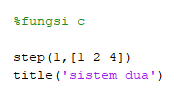
\includegraphics{7_c.png}
    \caption{Program M-file fungsi c}
    \label{soal_c}
\end{figure}
\begin{figure}[H]
    \centering
    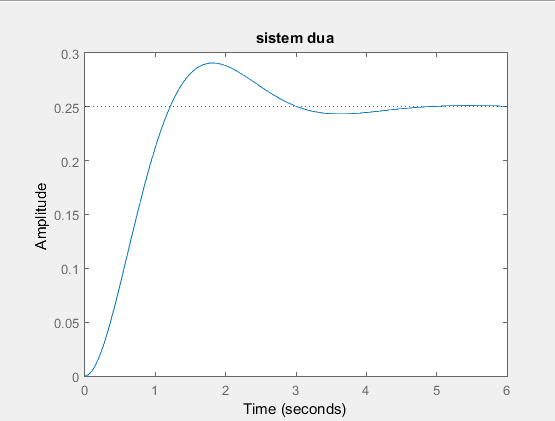
\includegraphics[width=\textwidth]{hasil_7_c.png}
    \caption{Keluaran plot MATLAB dari program fungsi c}
    \label{hasil_c}
\end{figure}

\subsubsection{fungsi empat}

\begin{figure}[H]
    \centering
    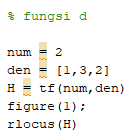
\includegraphics{7_d.png}
    \caption{Program M-file fungsi d}
    \label{soal_d}
\end{figure}
\begin{figure}[H]
    \centering
    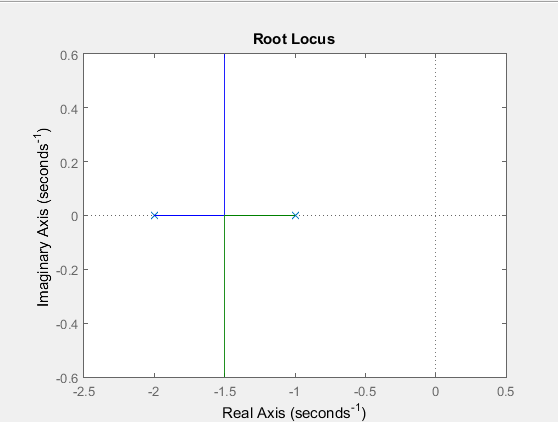
\includegraphics[width=\textwidth]{hasil_7_d.png}
    \caption{Keluaran plot MATLAB dari program fungsi d}
    \label{hasil_d}
\end{figure}

\section{Kesimpulan}

Dari percobaan pemodelan sistem diatas dapat disimpulnkan bahwa pemodelan dalam ilmu kendali memiliki peranan penting untuk mengetahui karakteristik dari masing-masing objek yang dimodelkan. pemodelan juga membantu untuk mempermudah penalaan pada sebuah sistem.

\end{document}
